\documentclass[a4paper, 12pt]{article}
\usepackage[T2A]{fontenc}
\usepackage[utf8]{inputenc}
\usepackage[english,russian]{babel}
\usepackage{amsmath, amsfonts, amssymb, amsthm, mathtools, misccorr, indentfirst, multirow}
\usepackage{wrapfig}
\usepackage{graphicx}
\usepackage{subfig}
\usepackage{adjustbox}
\usepackage{pgfplots}

\usepackage{geometry}
\geometry{top=20mm}
\geometry{bottom=20mm}
\geometry{left=20mm}
\geometry{right=20mm}
\newcommand{\angstrom}{\textup{\AA}}


\title{Лабораторная работа 2.1\\Опыт Франка-Герца}
\author{Нехаев Александр, гр. 654}
\date{\today}

\begin{document}
	\maketitle
	\pagenumbering{gobble}
	\newpage
	\pagenumbering{arabic}
	\tableofcontents
	\newpage
	\section{Введение}
	\paragraph{Цель работы} методом электронного возбуждения измерить энергию первого уровня атома гелия в динамическом и статическом режимах.
	\section{Теоретическое введение
		}
	Опыт Франка-Герца --- простой опыт, подтверждающий дискретность внутренней энергии атома. 
	Разреженный одноатомный газ (He) заполняет трёхэлектродную лампу. Электроны, испускаемые разогретым катодом, ускоряются в постоянном электрическом поле, созданным между катодом и сетчатым анодом лампы. Передвигаясь от катода к аноду, электроны сталкиваются с атомами гелия. Если энергия электрона недостаточна для того, чтобы перевести его в возбужденное состояние (или ионизировать), то возможны только упругие столкновения. По мере увеличения разности потенциалов энергия электронов увеличивается и оказывается достаточной для возбуждения атомов. При таких неупругих столкновениях кинетическая энергия электрона передаётся одному из атомных электронов, вызывая его переход на свободный энергетический уровень (возбуждение) или совсем отрывая его от атома (ионизация).
	Третьим электродом лампы является коллектор. Между ним и анодом поддерживается небольшое задерживающее напряжение. Ток коллектора измеряется микроамперметром.
	При увеличении потенциала анода ток в лампе вначале растет, а когда энергия электронов становится достаточной для возбуждения атомов, ток коллектора резко уменьшается, так как электроны почти полностью теряют свою энергию при неупругих соударениях с атомами. При дальнейшем увеличении потенциала анода ток коллектора вновь возрастает. Следующее замедление роста тока происходит в момент, когда часть электронов неупруго сталкивается с атомами два раза: первый раз посередине пути, второй -- у анода. Таким образом, на кривой зависимости тока коллектора от напряжения анода имеется ряд максимумов и минимумов, отстоящих друг от друга на равные расстояния $\Delta V$, равные энергии первого возбуждённого состояния.
	
	Теория, описывающая дискретность энергетических уровней атома He довольно сложная в плане вычислений, а концептуально всё сводится к решению уравнения Шрёдингера.
	
	Гамильтониан системы выглядит следующим образом
	
	\begin{equation}
		\hat{H}=-\frac{\hbar^2}{2m}\Delta_1-\frac{\hbar^2}{2m}\Delta_2-\frac{Ze^2}{4\pi\varepsilon r_1}-\frac{Ze^2}{4\pi\varepsilon r_2}+\frac{e^2}{4\pi\varepsilon r_{12}}
	\end{equation}
	
	Решить требуется стационарное уравнение Шрёдингера
	
	\begin{equation}
		\hat{H}\Psi({\bf r}_1,\,{\bf r}_2)=E\Psi({\bf r}_1,\,{\bf r}_2)
	\end{equation}
	
	Гамильтониан можно переписать в виде
	
	\begin{equation}
		\hat{H}=\hat{H}_1+\hat{H}_2+V_{12},
	\end{equation}
	
	где $V_{12}$ описывает взаимодействие электронов, которым традиционно пренебрегают, разделяют переменные и решают одноэлектронные уравнения Шрёдингера, получая приблизительную волновую функцию, затем используя соображения о принципе запрета Паули и т.д. учитывают спин электронов и делают поправки на их взаимодействие. Описание этой процедуры выходит за рамки работы, поэтому нет нужды описывать её подробно.
	\section{Экспериментальная часть}
		Сначала исследуем ВАХ в динамическом режиме. Для трех значений задерживающего напряжения получим осциллограммы. Важно заметить, что развертка осуществляется справа налево. Цена деления осциллографа 5В.
	\begin{figure}[h!]
		\minipage{0.32\textwidth}
			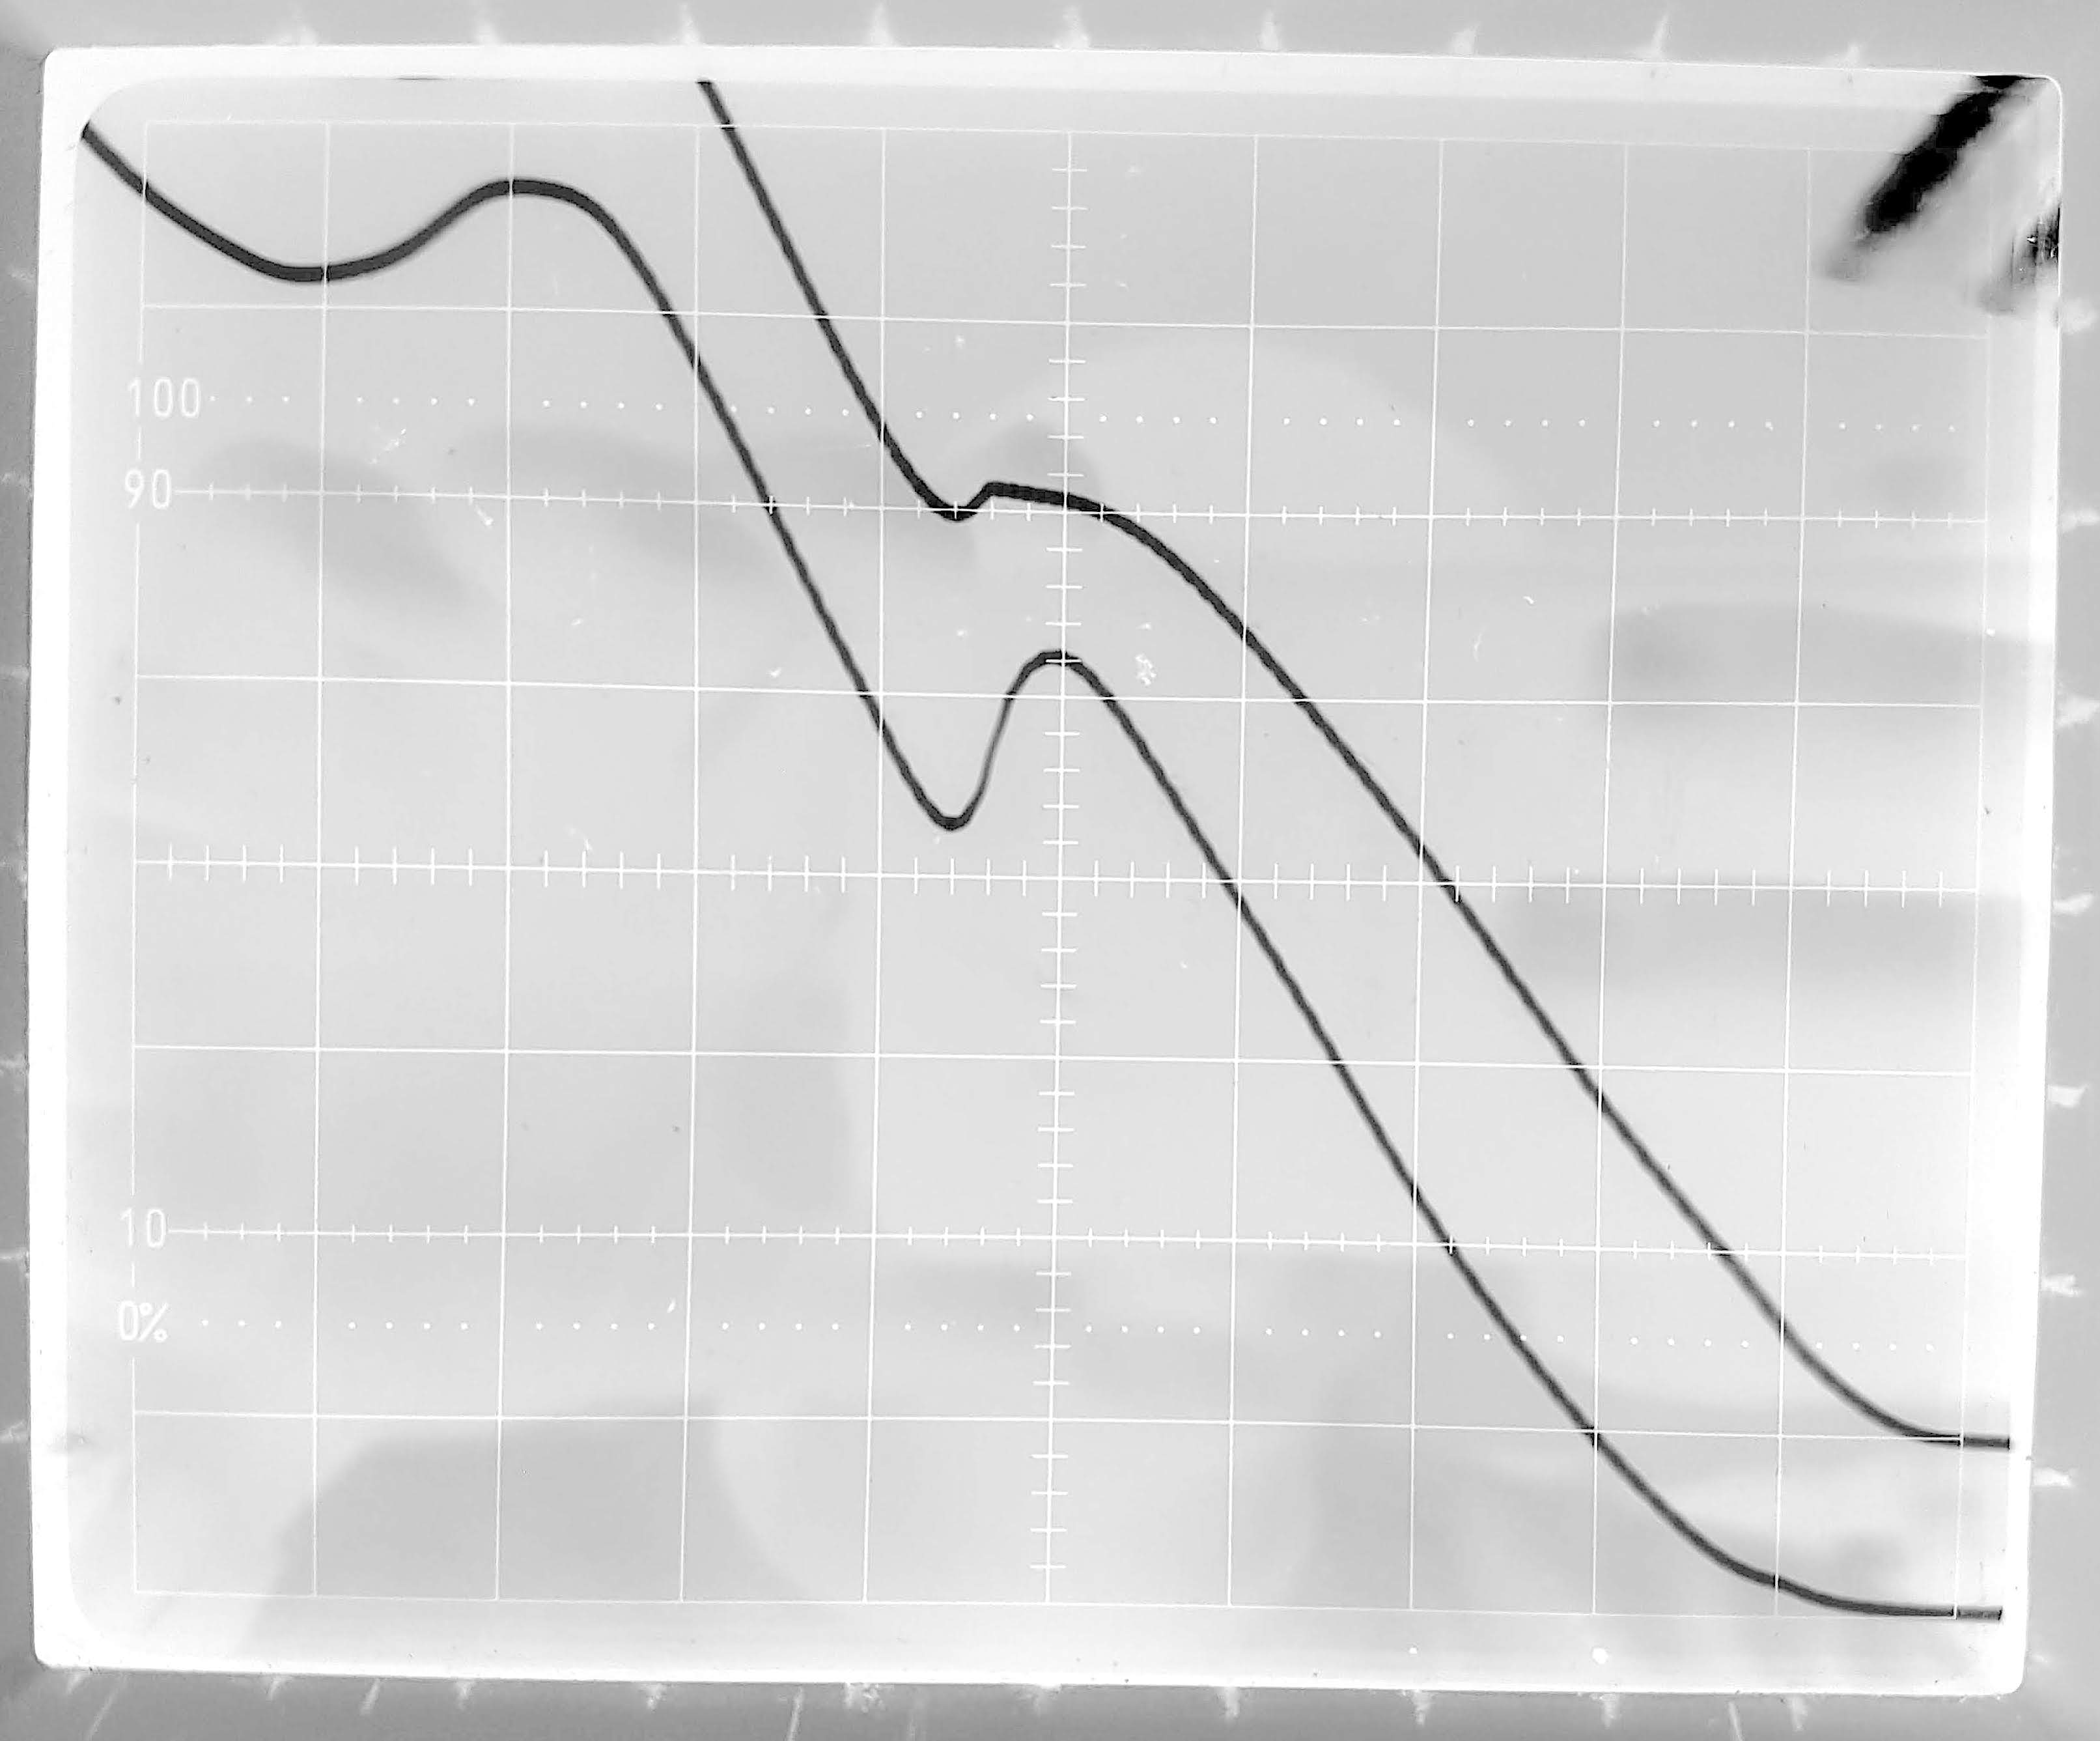
\includegraphics[width=\linewidth]{20181011_100150.jpg}
			\caption{$U=4$В}
		\endminipage\hfill
		\minipage{0.32\textwidth}
			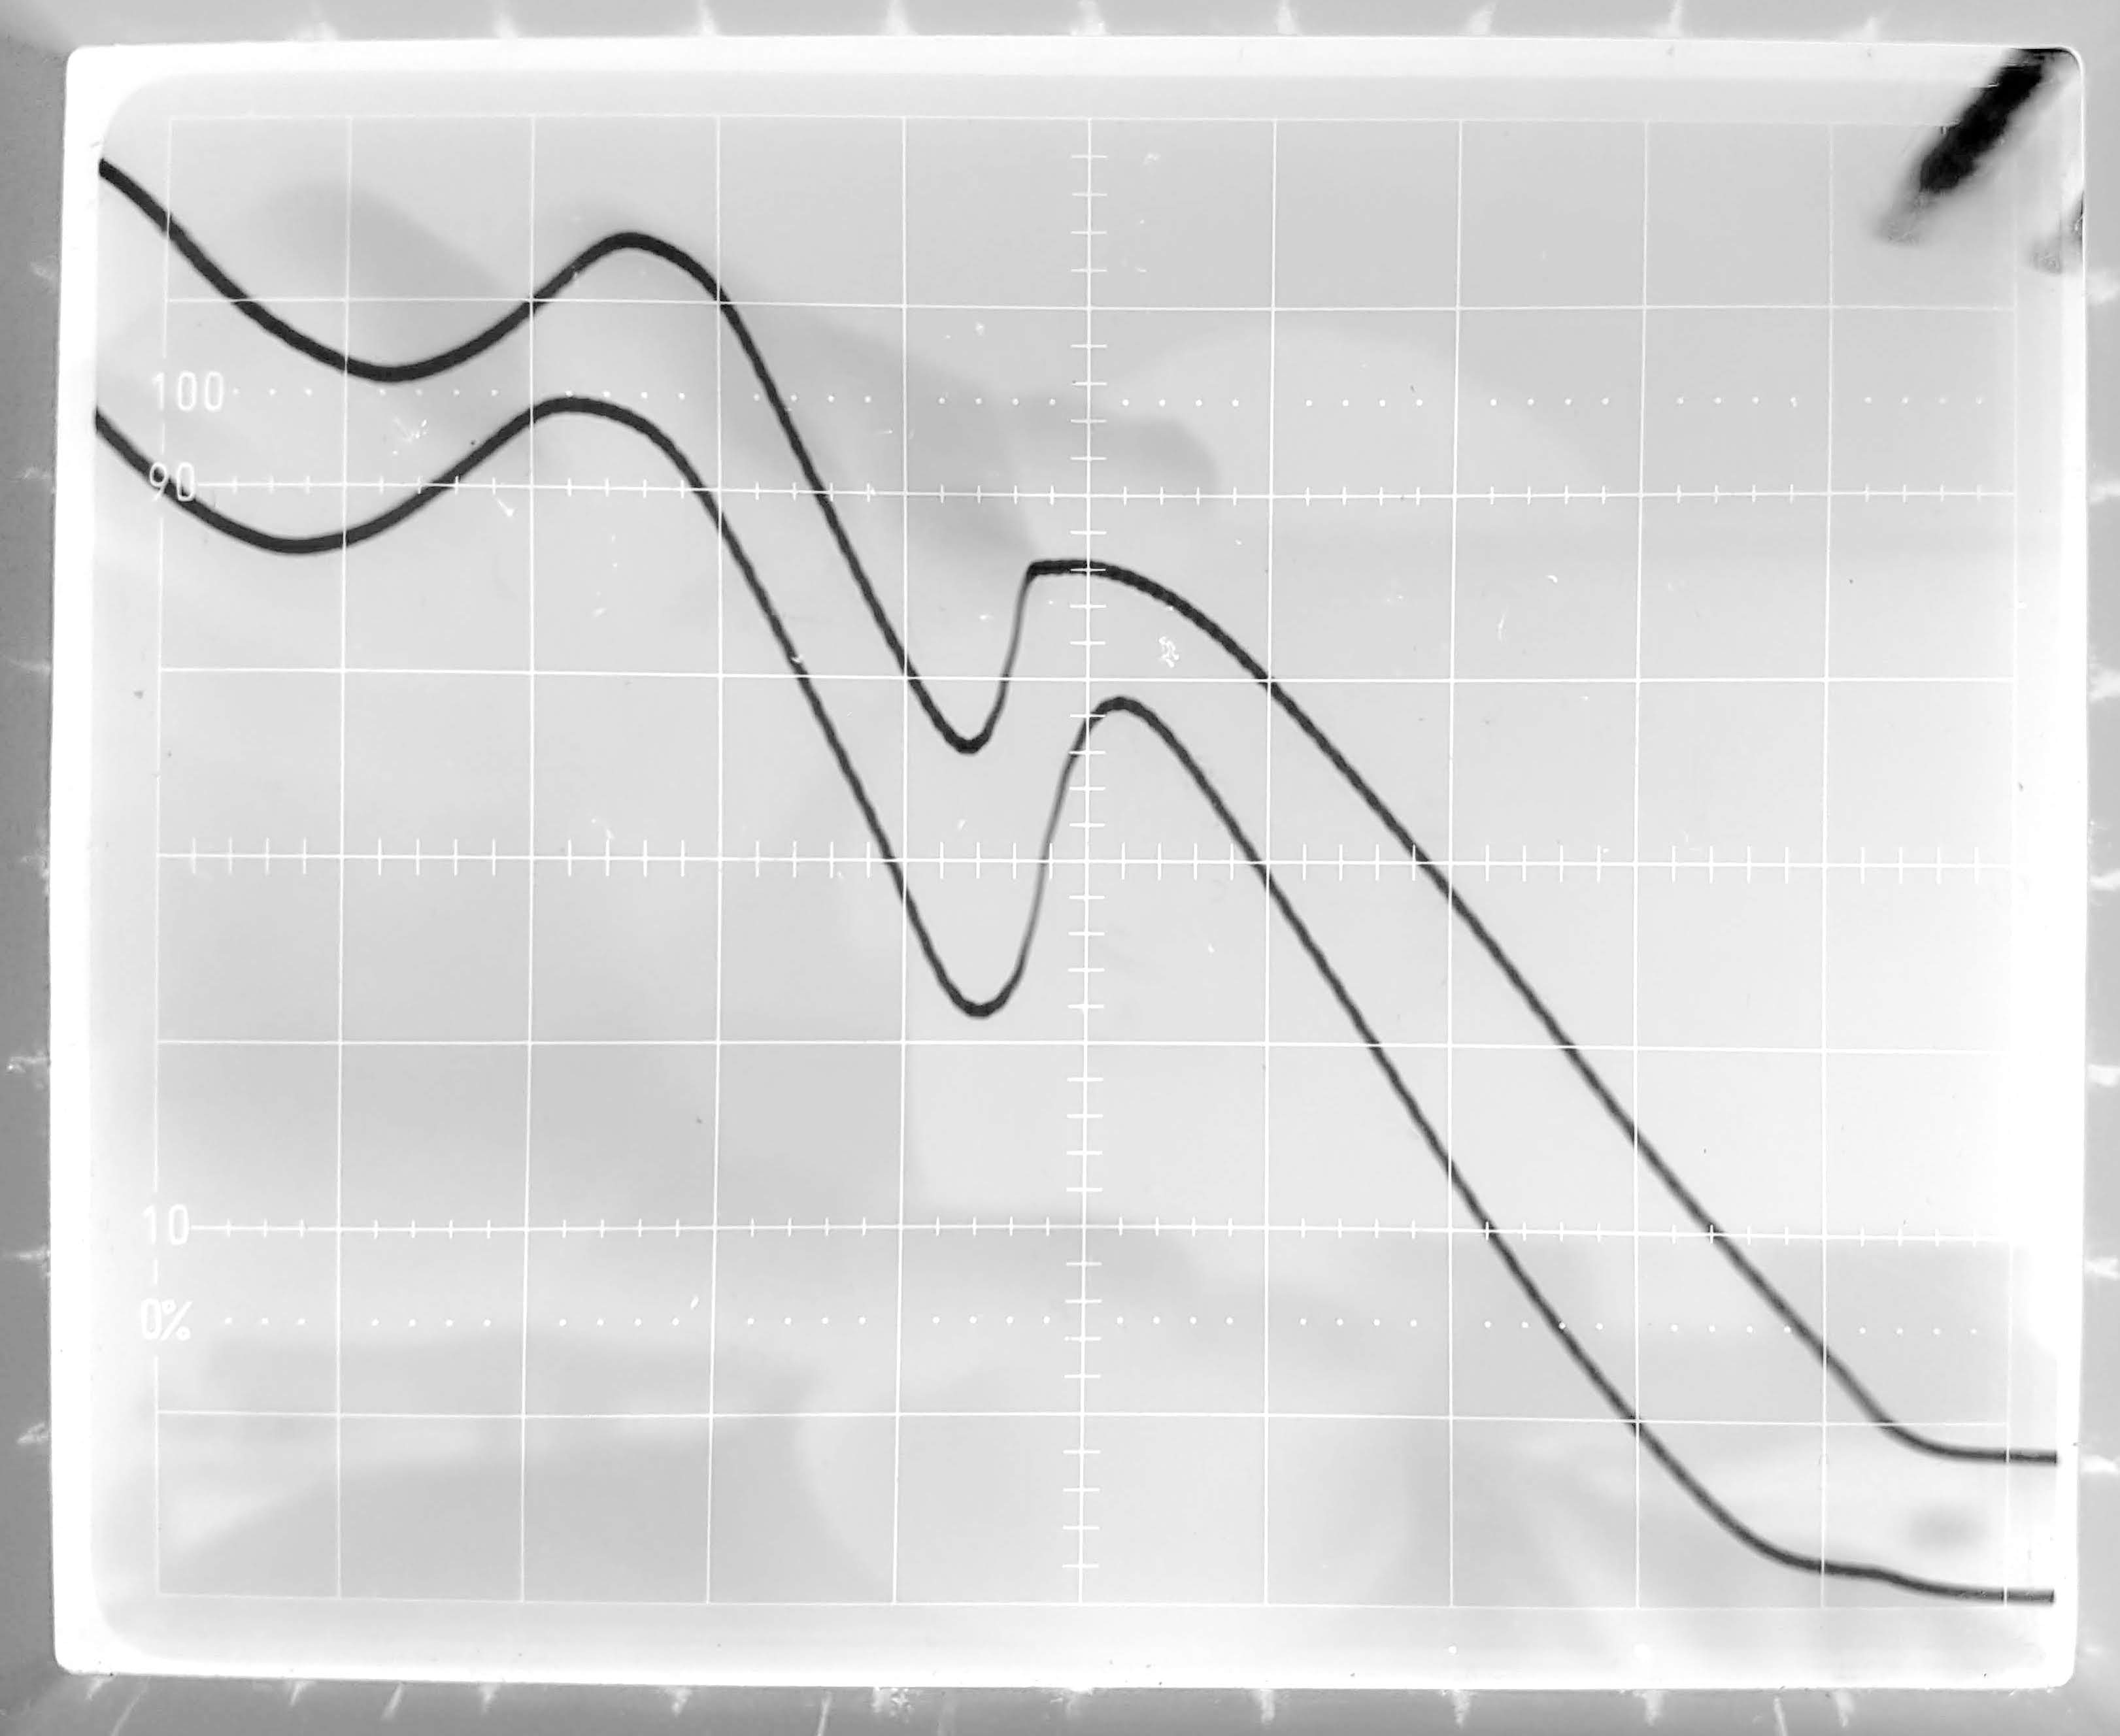
\includegraphics[width=\linewidth]{20181011_100218.jpg}
			\caption{$U=6$В}
		\endminipage\hfill
		\minipage{0.32\textwidth}
			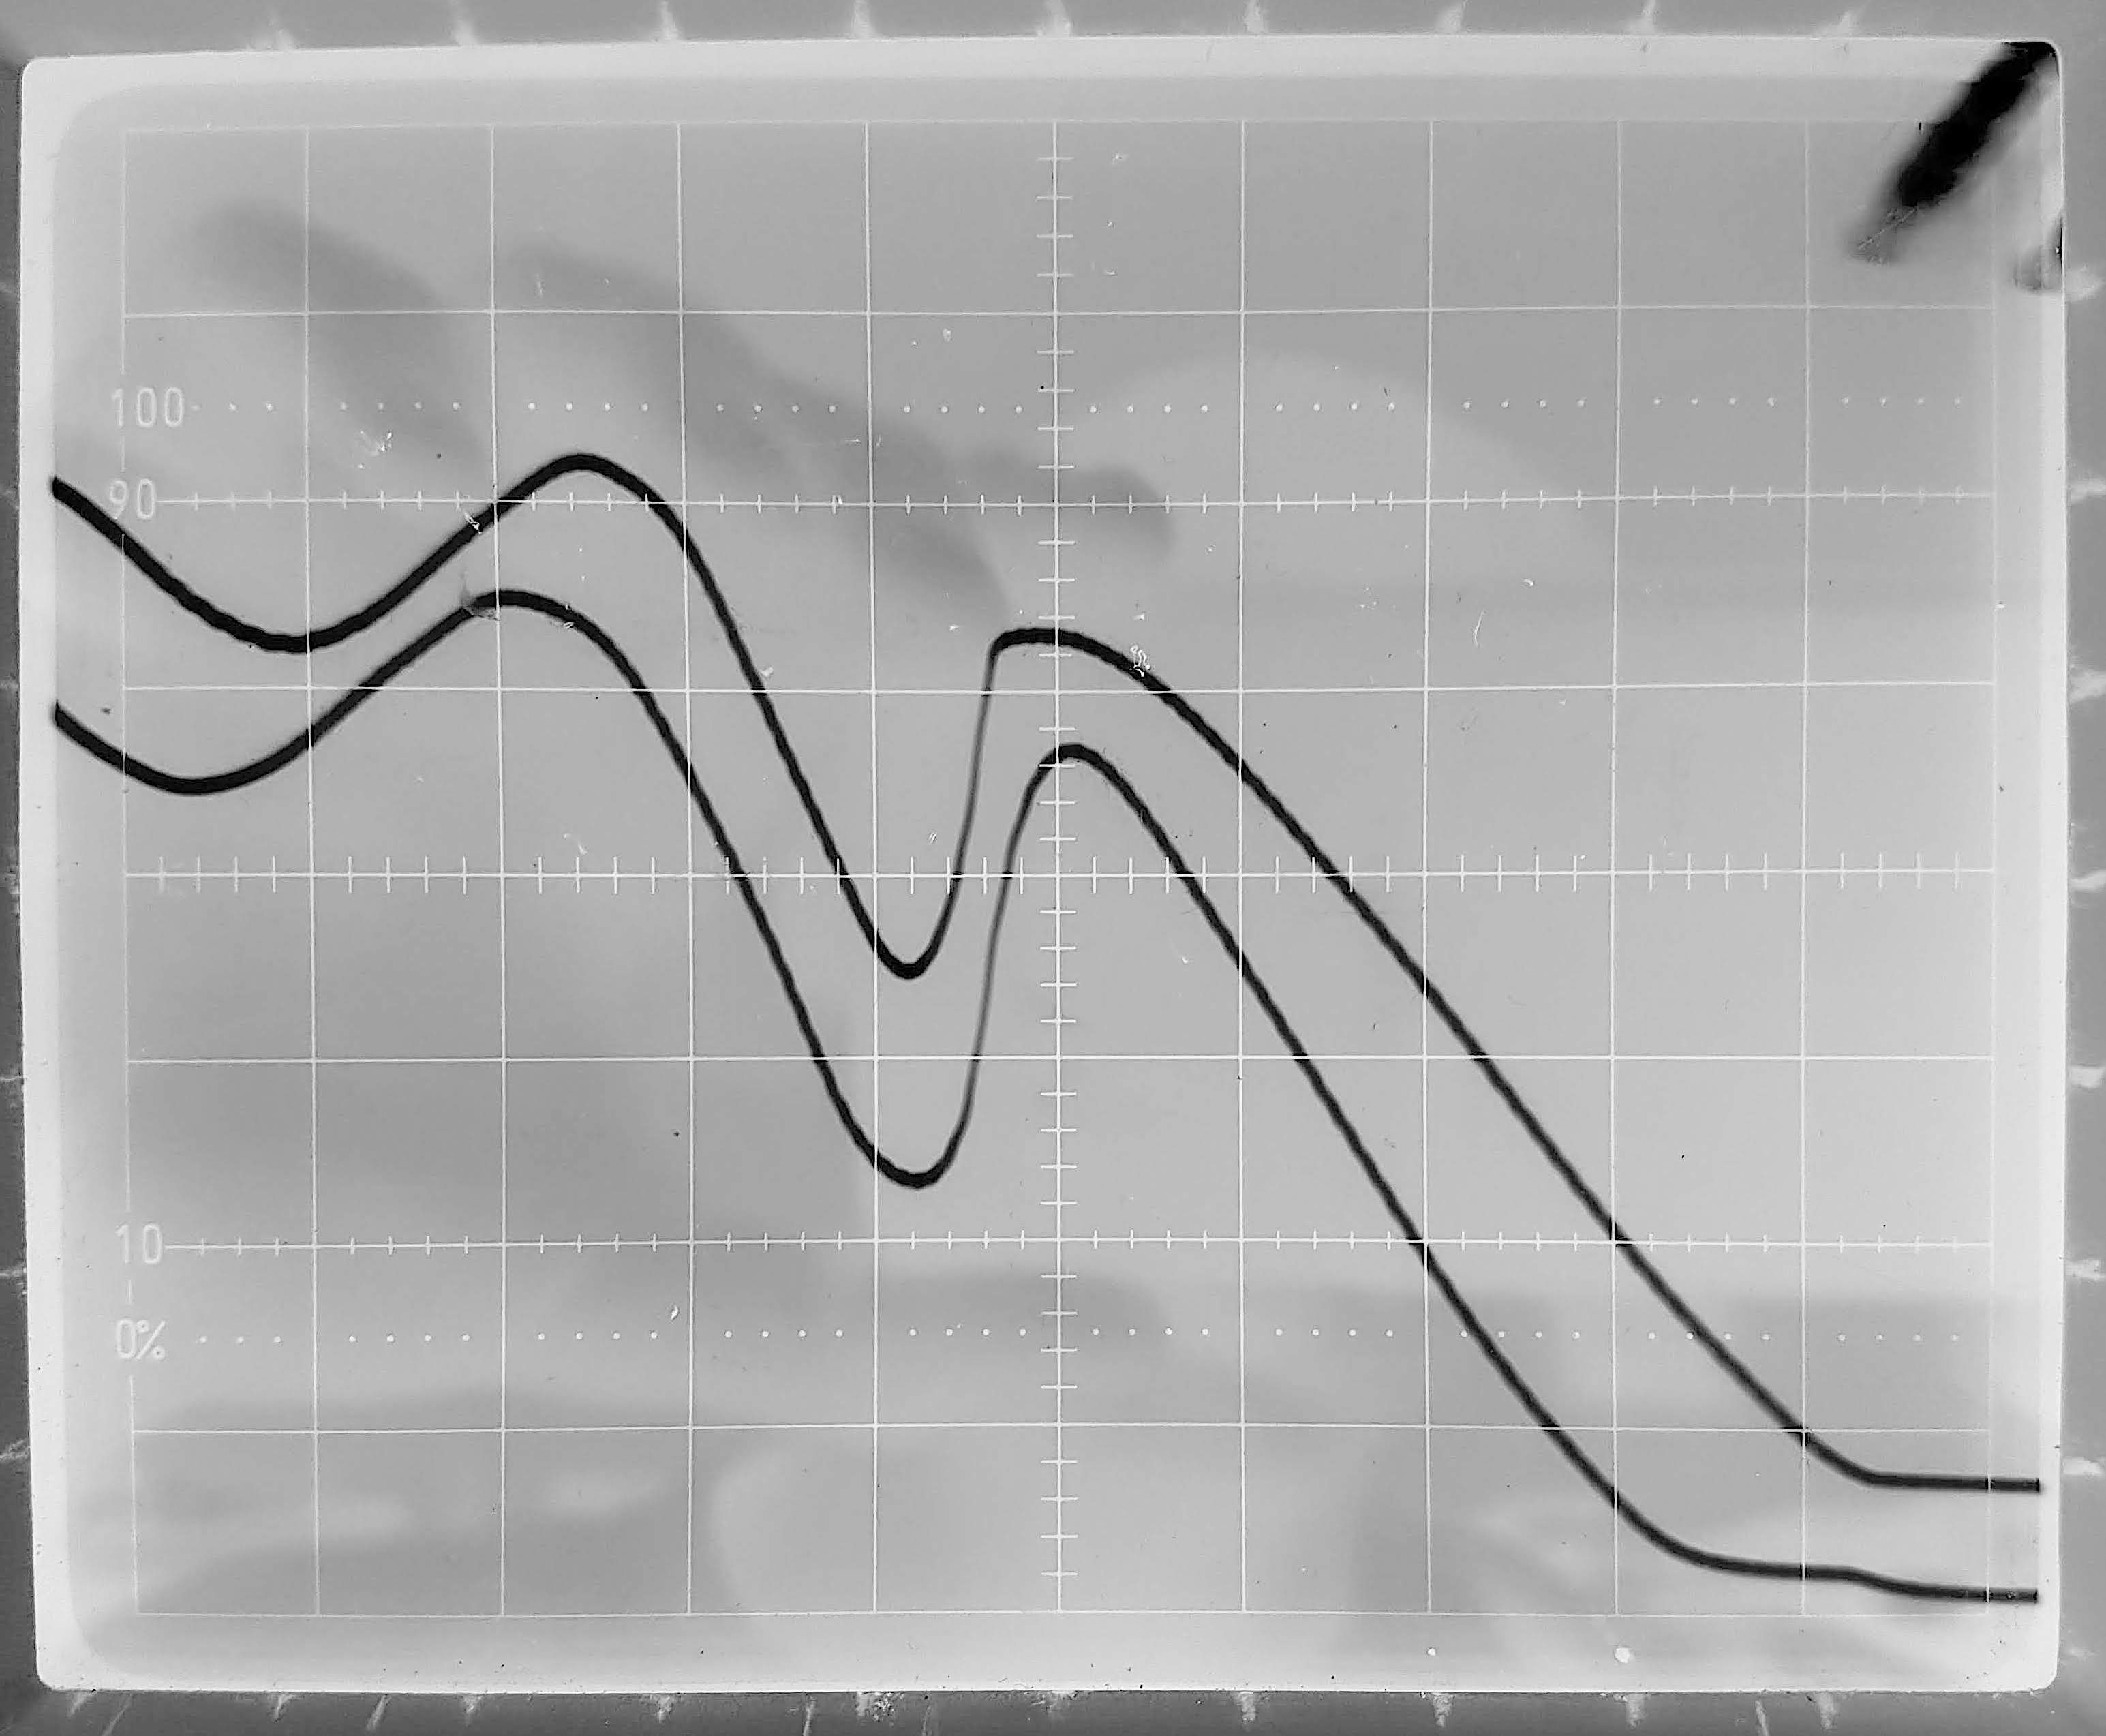
\includegraphics[width=\linewidth]{20181011_100245.jpg}
			\caption{$U=8$В}
		\endminipage
	\end{figure}
	
	Затем, исследуем ВАХ более подробно, перейдя в статический режим.
	\begin{figure}[!h]
		\begin{tikzpicture}
			\begin{axis}[
			title={$U=4,6,8$, В},
			xlabel={$U,\ \text{В}$},
			ylabel={о. е.},
			xmin=0.0,
			xmax=80.0,
			ymin=0.0,
			ymax=75.0,
			ymajorgrids=true,
			xmajorgrids=true,
			grid style=dashed,
			width=\textwidth,
			height=13cm,
			]
			\addplot+[
				color=black,
				error bars/.cd,
				y dir=both, y explicit,
				x dir=both, x explicit
			]
			coordinates{
			(2, 1.5)+-(0.5,0.5)
			(4, 2.67)+-(0.5,0.5)
			(6, 3.68)+-(0.5,0.5)
			(8, 4.95)+-(0.5,0.5)
			(10, 6.08)+-(0.5,0.5)
			(12, 7.15)+-(0.5,0.5)
			(14, 8.23)+-(0.5,0.5)
			(16, 9.15)+-(0.5,0.5)
			(18, 10.02)+-(0.5,0.5)
			(20, 10.67)+-(0.5,0.5)
			(22, 11.6)+-(0.5,0.5)
			(24, 12.37)+-(0.5,0.5)
			(26, 13.29)+-(0.5,0.5)
			(28, 14.16)+-(0.5,0.5)
			(30, 14.9)+-(0.5,0.5)
			(32, 15.81)+-(0.5,0.5)
			(34, 16.79)+-(0.5,0.5)
			(36, 17.56)+-(0.5,0.5)
			(38, 18.6)+-(0.5,0.5)
			(38, 24.74)+-(0.5,0.5)
			(40, 19.12)+-(0.5,0.5)
			(42, 21.33)+-(0.5,0.5)
			(44, 27.6)+-(0.5,0.5)
			(45, 23.08)+-(0.5,0.5)
			(46, 28.19)+-(0.5,0.5)
			(48, 28.95)+-(0.5,0.5)
			(50, 29.55)+-(0.5,0.5)
			(52, 30.37)+-(0.5,0.5)
			(54, 31.1)+-(0.5,0.5)
			(56, 31.67)+-(0.5,0.5)
			(58, 32.5)+-(0.5,0.5)
			(60, 33.4)+-(0.5,0.5)
			(62, 33.88)+-(0.5,0.5)
			(62, 40.95)+-(0.5,0.5)
			(64, 35.03)+-(0.5,0.5)
			(66, 51.71)+-(0.5,0.5)
			(68, 54.09)+-(0.5,0.5)
			(70, 55.55)+-(0.5,0.5)
			(72, 57.12)+-(0.5,0.5)
			(74, 61.15)+-(0.5,0.5)
			(76, 69.02)+-(0.5,0.5)
			};
			\addplot+[
				color=black,
				error bars/.cd,
				y dir=both, y explicit,
				x dir=both, x explicit
			]
			coordinates{
				(2.69, 2)+-(0.5,0.5)
				(4.25, 4)+-(0.5,0.5)
				(6.16, 7)+-(0.5,0.5)
				(8.08, 11)+-(0.5,0.5)
				(10.1, 15)+-(0.5,0.5)
				(12.24, 20)+-(0.5,0.5)
				(14.13, 25)+-(0.5,0.5)
				(16.33, 30)+-(0.5,0.5)
				(18.34, 35)+-(0.5,0.5)
				(20.33, 39)+-(0.5,0.5)
				(22.3, 41)+-(0.5,0.5)
				(24.29, 28)+-(0.5,0.5)
				(26.44, 27)+-(0.5,0.5)
				(28.3, 33)+-(0.5,0.5)
				(30.03, 38)+-(0.5,0.5)
				(32.75, 47)+-(0.5,0.5)
				(34.6, 52)+-(0.5,0.5)
				(36.59, 54)+-(0.5,0.5)
				(38.77, 55)+-(0.5,0.5)
				(40.4, 53)+-(0.5,0.5)
				(42.5, 50)+-(0.5,0.5)
				(44.42, 48)+-(0.5,0.5)
				(46.39, 47)+-(0.5,0.5)
				(48.6, 47)+-(0.5,0.5)
				(50.68, 48)+-(0.5,0.5)
				(52.01, 49)+-(0.5,0.5)
				(54.31, 51)+-(0.5,0.5)
				(56.33, 53)+-(0.5,0.5)
				(58.49, 55)+-(0.5,0.5)
				(60.79, 56)+-(0.5,0.5)
				(62.35, 57)+-(0.5,0.5)
				(64.44, 56)+-(0.5,0.5)
				(68.15, 57)+-(0.5,0.5)
			};
			\addplot+[
				color=black,
				error bars/.cd,
				y dir=both, y explicit,
				x dir=both, x explicit
			]
			coordinates{
				(2.97, 0)+-(0.5,0.5)
				(4.29, 1)+-(0.5,0.5)
				(6.37, 4)+-(0.5,0.5)
				(8.34, 8)+-(0.5,0.5)
				(10.08, 11)+-(0.5,0.5)
				(12.55, 17)+-(0.5,0.5)
				(14.48, 22)+-(0.5,0.5)
				(16.01, 25)+-(0.5,0.5)
				(18.31, 30)+-(0.5,0.5)
				(20.7, 35)+-(0.5,0.5)
				(22.9, 39)+-(0.5,0.5)
				(24.46, 40)+-(0.5,0.5)
				(26.2, 17)+-(0.5,0.5)
				(28.25, 19)+-(0.5,0.5)
				(30.32, 25)+-(0.5,0.5)
				(32.33, 32)+-(0.5,0.5)
				(34.28, 38)+-(0.5,0.5)
				(36.37, 42)+-(0.5,0.5)
				(38.07, 44)+-(0.5,0.5)
				(40.17, 42)+-(0.5,0.5)
				(42.58, 40)+-(0.5,0.5)
				(44.17, 38)+-(0.5,0.5)
				(46.14, 35)+-(0.5,0.5)
				(48.47, 33)+-(0.5,0.5)
				(50.32, 33)+-(0.5,0.5)
				(52.38, 34)+-(0.5,0.5)
				(54.37, 36)+-(0.5,0.5)
				(56.56, 38)+-(0.5,0.5)
				(58.79, 39)+-(0.5,0.5)
				(62.41, 40)+-(0.5,0.5)
				(64.6, 40)+-(0.5,0.5)
				(65.06, 40)+-(0.5,0.5)
				(68.28, 39)+-(0.5,0.5)
				(68.5, 39)+-(0.5,0.5)
				};
				\addlegendentry{$U=4$ В}
				\addlegendentry{$U=6$ В}
				\addlegendentry{$U=8$ В}
			\end{axis}
		\end{tikzpicture}
	\end{figure}
	
	\begin{table}[!htb]
		\minipage{0.32\textwidth}
			\begin{tabular}{|c|c|c|}
			\hline
			№ & $V$, В & $I$, В\\
			\hline
 			1 & 2 & 1.5 \\
 			 2 & 4 & 2.67 \\
 			 3 & 6 & 3.68 \\
 			 4 & 8 & 4.95 \\
 			 5 & 10 & 6.08 \\
 			 6 & 12 & 7.15 \\
 			 7 & 14 & 8.23 \\
 			 8 & 16 & 9.15 \\
 			 9 & 18 & 10.02 \\
 			 10 & 20 & 10.67 \\
 			 11 & 22 & 11.6 \\
 			 12 & 24 & 12.37 \\
 			 13 & 26 & 13.29 \\
 			 14 & 28 & 14.16 \\
 			 15 & 30 & 14.9 \\
 			 16 & 32 & 15.81 \\
 			 17 & 34 & 16.79 \\
 			 18 & 36 & 17.56 \\
 			 19 & 38 & 18.6 \\
 			 20 & 38 & 24.74 \\
 			 21 & 40 & 19.12 \\
 			 22 & 42 & 21.33 \\
 			 23 & 44 & 27.6 \\
 			 24 & 45 & 23.08 \\
 			 25 & 46 & 28.19 \\
 			 26 & 48 & 28.95 \\
 			 27 & 50 & 29.55 \\
 			 28 & 52 & 30.37 \\
 			 29 & 54 & 31.1 \\
 			 30 & 56 & 31.67 \\
 			 31 & 58 & 32.5 \\
 			 32 & 60 & 33.4 \\
 			 33 & 62 & 33.88 \\
 			 34 & 62 & 40.95 \\
 			 35 & 64 & 35.03 \\
 			 36 & 66 & 51.71 \\
 			 37 & 68 & 54.09 \\
 			 38 & 70 & 55.55 \\
 			 39 & 72 & 57.12 \\
 			 40 & 74 & 61.15 \\
 			 41 & 76 & 69.02 \\
 			\hline
			\end{tabular}
			\caption{$U=4$В}
		\endminipage\hfill
		\minipage{0.32\textwidth}
			\begin{tabular}{|c|c|c|}
			\hline
			№ & $V$, В & $I$, В\\
			\hline
			1 & 2.69 & 2 \\
 			2 & 4.25 & 4 \\
 			3 & 6.16 & 7 \\
 			4 & 8.08 & 11 \\
 			5 & 10.1 & 15 \\
 			6 & 12.24 & 20 \\
 			7 & 14.13 & 25 \\
 			8 & 16.33 & 30 \\
 			9 & 18.34 & 35 \\
 			10 & 20.33 & 39 \\
 			11 & 22.3 & 41 \\
 			12 & 24.29 & 28 \\
 			13 & 26.44 & 27 \\
 			14 & 28.3 & 33 \\
 			15 & 30.03 & 38 \\
 			16 & 32.75 & 47 \\
 			17 & 34.6 & 52 \\
 			18 & 36.59 & 54 \\
 			19 & 38.77 & 55 \\
 			20 & 40.4 & 53 \\
 			21 & 42.5 & 50 \\
 			22 & 44.42 & 48 \\
 			23 & 46.39 & 47 \\
 			24 & 48.6 & 47 \\
 			25 & 50.68 & 48 \\
 			26 & 52.01 & 49 \\
 			27 & 54.31 & 51 \\
 			28 & 56.33 & 53 \\
 			29 & 58.49 & 55 \\
 			30 & 60.79 & 56 \\
 			31 & 62.35 & 57 \\
 			32 & 64.44 & 56 \\
 			33 & 68.15 & 57 \\
			\hline
			\end{tabular}
			\caption{$U=6$В}
		\endminipage\hfill
		\minipage{0.32\textwidth}
			\begin{tabular}{|c|c|c|}
			\hline
			№ & $V$, В & $I$, В\\
			\hline
			1 & 2.97 & 0 \\
 			2 & 4.29 & 1 \\
 			3 & 6.37 & 4 \\
 			4 & 8.34 & 8 \\
 			5 & 10.08 & 11 \\
 			6 & 12.55 & 17 \\
 			7 & 14.48 & 22 \\
 			8 & 16.01 & 25 \\
 			9 & 18.31 & 30 \\
 			10 & 20.7 & 35 \\
 			11 & 22.9 & 39 \\
 			12 & 24.46 & 40 \\
 			13 & 26.2 & 17 \\
 			14 & 28.25 & 19 \\
 			15 & 30.32 & 25 \\
 			16 & 32.33 & 32 \\
 			17 & 34.28 & 38 \\
 			18 & 36.37 & 42 \\
 			19 & 38.07 & 44 \\
 			20 & 40.17 & 42 \\
 			21 & 42.58 & 40 \\
 			22 & 44.17 & 38 \\
 			23 & 46.14 & 35 \\
 			24 & 48.47 & 33 \\
 			25 & 50.32 & 33 \\
 			26 & 52.38 & 34 \\
 			27 & 54.37 & 36 \\
 			28 & 56.56 & 38 \\
 			29 & 58.79 & 39 \\
 			30 & 62.41 & 40 \\
 			31 & 64.6 & 40 \\
 			32 & 65.06 & 40 \\
 			33 & 68.28 & 39 \\
 			34 & 68.5 & 39 \\
			\hline
			\end{tabular}
			\caption{$U=8$В}
		\endminipage
	\end{table}
	\newpage
	Значения пиков для статического режима, определенные по графику вынесем в таблицу:
	\begin{table}[!htb]
		\caption{Статический режим}
		\centering
		\begin{tabular}{|c|c|c|c|c|c|c|}
			\hline
			$U,\ V$ & $V_{\text{max 1}}$ & $V_{\text{max 2}}$ & $\Delta V_{\text{max}}$ & $V_{\text{min 1}}$ & $V_{\text{min 2}}$ & $\Delta V_{\text{min}}$\\
			\hline
			4 & $44 \pm 0.5$ & $76 \pm 0.5$ & $32 \pm 0.7$ & $40 \pm 0.5$ & $45 \pm 0.5$ & $5 \pm 0.7$ \\
		 	6 & $38.77 \pm 0.5$ & $62.35 \pm 0.5$ & $23.58 \pm 0.7$ & $26.44 \pm 0.5$ & $46.39 \pm 0.5$ & $19.95 \pm 0.7$ \\
 			8 & $38.07 \pm 0.5$ & $62.41 \pm 0.5$ & $24.34 \pm 0.7$ & $26.2 \pm 0.5$ & $48.47 \pm 0.5$ & $22.27 \pm 0.7$ \\
 			\hline
		\end{tabular}
	\end{table}
	\begin{table}[h!]
			\centering
			\caption{Табличные значения для атома гелия}
			\label{table3}
			\begin{tabular}{|c|c|}
				\hline
				$E_I$                                  & 24,47 эВ \\ \hline
				$E_1$ & 19,82 эВ \\ \hline
			\end{tabular}
		\end{table}
	\section{Вывод}
	Проделанная работа позволяет убедится в дискретности энергетических уровней в атоме гелия. Снятие вольт-амперной характеристики в динамическом режиме позволяет наглядно увидеть структуру энергетических уровней. Статический режим же нужен для более точного измерения энергии возбуждения атома. Эксперимент показал, что измеренная нами энергия атома близка к табличной(сходится по порядку величины) Из-за неправильной постановки эксперимента не смогли получить правильный график для $U=4$ В.
\end{document}